% ##############################################################################
\chapter{Présentation générale}
%Présentation de GK (ie contexte organisationnel)
%	Métiers (Eau, Médecine, ...)
%	Organisation générale (Logistique = support)
%	Environnement du produit
%	Caractéristiques des éléments de l'environnement
% ==============================================================================
\section{Introduction}
Ce document constitue le cahier des charges du projet de système de gestion des transports au bénéfice de la société \mo réalisé par l'assistance à maîtrise d'ouvrave \amo.
% Fin de la section [Introduction]
% ==============================================================================

% ==============================================================================
\section{\mo}
% ------------------------------------------------------------------------------
\subsection{Présentation}
Avec des dizaines de millions de volontaires dans 187 sociétés internationales, \mo est l'une des plus grandes organisations humanitaires au monde. Elle agit avant, pendant et après les catastrophes et les urgences relatives à la santé pour répondre aux besoins des plus vulnérables et pour améliorer leur vie. Elle dispense cette aide sans distinction de nationalité, de race, de religion, de classe ou d'opinions politiques.
\\
Elle puise sa force de son réseau de volontaires, de l'expertise basée dans la communauté et de sa capacité à donner une voix mondiale aux personnes vulnérables. Elle travaille en tant que partenaire dans le développement, la réponse aux catastrophes, l'aide pour une vie saine et sure, et l'amélioration des normes humanitaires. Le résultat : Elle aide à réduire les vulnérabilités, et rend les communautés plus résistantes.
% Fin de la sous-section [Présentation]
% ------------------------------------------------------------------------------

% ------------------------------------------------------------------------------
\subsection{Métiers}
\mo est divisé en 5 métiers :
\begin{itemize}
	\item Médecine
	\item Eau et sanitaire
	\item Distribution
	\item Logistique
	\item Télécoms
\end{itemize}
Leur dépendances respéctives sont décrites dans la Fig. \ref{dep}
\vspace{1cm}
\begin{figure}
\centering
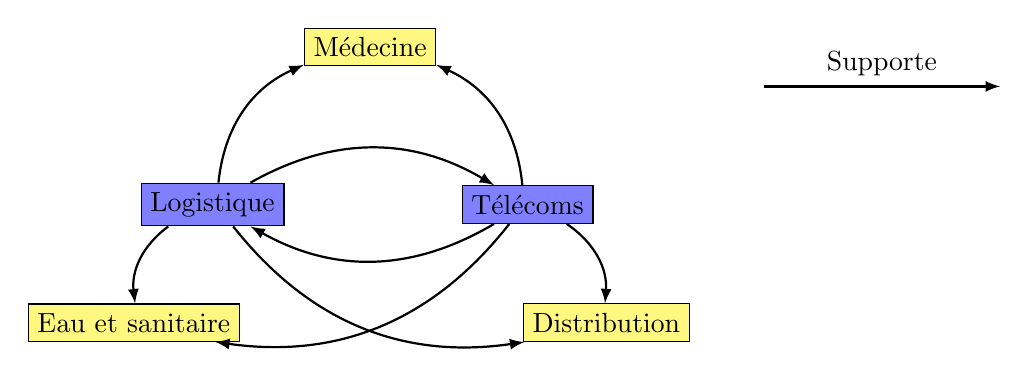
\begin{tikzpicture}
% définition des styles
\tikzstyle{metier}=[rectangle,draw,fill=yellow!50,text=black]
\tikzstyle{support}=[rectangle,draw,fill=blue!50,text=black]
\tikzstyle{supporte}=[->,>=latex,thick,rounded corners=4pt]
% les nœuds
\node[metier] (e) at (-3,-3) {Eau et sanitaire};
\node[metier] (m) at (0,0.5) {Médecine};
\node[metier] (d) at (3,-3) {Distribution};
\node[support] (l) at (-2,-1.5) {Logistique};
\node[support] (t) at (2,-1.5) {Télécoms};
% les flèches
\draw[supporte] (l) to[bend left] (t);
\draw[supporte] (l) to[bend right] (e);
\draw[supporte] (l) to[bend left] (m);
\draw[supporte] (l) to[bend right] (d);
\draw[supporte] (t) to[bend left] (l);
\draw[supporte] (t) to[bend left] (e);
\draw[supporte] (t) to[bend right] (m);
\draw[supporte] (t) to[bend left] (d);
% la légende
\draw[supporte] (5,0) -- (8,0) node[midway,above]{Supporte};
\end{tikzpicture}
\caption{Dépendances entre les métiers}
\label{dep}
\end{figure}
% Fin de la sous-section [Métiers]
% ------------------------------------------------------------------------------

% Fin de la section [\mo]
% ==============================================================================

% ==============================================================================
\section{Environnement du produit recherché}
Cette section décrit les conditions de fonctionnement de la solution recherchée.

%-------------------------------------------------------------------------------
\subsection{Listes exhaustives des éléments et contraintes}

\subsubsection{Personnes}
Les utilisateurs seront :
\begin{itemize}
\item Le secrétariat central
\item Les logisticiens sur le terrain
\item Les métiers
\end{itemize}

\subsubsection{Équipement}
\mo possède déjà une infrastructure informatique, constituée de machines serveurs et clientes, comme suit :
\begin{itemize}
\item Les serveurs tournent sur un système Microsoft Windows mais une migration est prévue sur GNU/Linux. Le stockage des données est pris en charge par deux SGBDR que sont MySql Server et Oracle.
\item Les clients sont :
\begin{itemize}
\item Ordinateurs portables : sous Microsoft Windows 7 équipés de 16 Go de mémoire vive et de 250 Go d'espace disque. Microsoft Internet Explorer et Mozilla Firefox sont les deux navigateurs présents par défaut et leur utilisation est fonction des préférences de l'utilisateur.
\item Smartphones : sous Androïd.
\end{itemize}
\end{itemize}

\subsubsection{Contraintes}
La communication entre clients et serveur est assurée par une liaison réseau dépendant du lieu de l'intervention et pouvant reposer sur trois infrastructures (classé ici par ordre décroissant de préférence d'utilisation) :
\begin{itemize}
\item Internet (ADSL)
\item Téléphonique (GSM)
\item Satellitaire
\end{itemize}
Les lois étant différentes en fonction du pays où \mo intervient, il conviendra de prendre en compte les obligations cryptographiques en vigueur lors des échanges.
% Fin de la section [Environnement du produit recherché]
% ==============================================================================

% ==============================================================================
\section{Caractéristiques pour chaque élément de l'environnement}
\mo possèdent des équipes de spécialistes formés aux interventions d'urgence dans le cadre notamment de catastrophes naturelles (tsunamis, tremblements de terre...).
Cinq domaines de compétence y sont représentés :
\begin{itemize}
\item Médecine
\item Eau et sanitaire
\item Distribution
\item Logistique
\item Télécoms
\end{itemize}
% - - - - - - - - - - - - - - - - - - - - - - - - - - - - - - - - - - - - - - - 
\subsubsection{La logistique}
L'efficacité de l'aide apportée aux populations sinistrées repose en particulier sur celle des processus logistiques. De ce fait, la logistique apparaît comme un service support aux métiers (secteur médical, distribution, eau et sanitaires), sans lequel ils ne peuvent accomplir leurs missions.
\\
Actuellement, la logistique présente des complications :
\begin{itemize}
\item Communication \& partage d'informations peu efficaces
\item Redondance d'informations
\item Contraintes techniques \& environnementales
\item La location de matériel donne lieu à la création de documents qui sont jusqu'à présent réalisés manuellement.
\end{itemize}

\paragraph{Processus et fonctions clefs de la logistique}
Différents processus concourent à l'accomplissement des missions logistiques dont (liste non exhaustive) :
\begin{itemize}
\item Le processus d'achat
\item Le processus de stockage
\item Le processus de transport
\end{itemize}
L'ensemble des processus doit permettre de répondre aux fonctions clefs de la logistique que sont notamment :
\begin{itemize}
\item Planification/évaluation
\item Acquisition/achat
\item Organisation des transports
\item Gestion des entrepôts
\item Faire le suivi et rendre compte
\item Standardisation
\item Formation et renforcement des capacités
\end{itemize}

\paragraph{La chaîne logistique en situation d'urgence}

\paragraph{Les logisticiens de terrain}
En général, les équipes de logisticiens restent de dimension réduite (cinq à six personnes, dont un chef d'équipe), avec des profils spécialisés qui assurent en particulier des activités telles que :
\begin{itemize}
\item La mise en place et le maintien des procédures logistiques standards
\item L'achat des biens et des services
\item La facilitation de l'importation et l'exportation des marchandises
\item L'organisation du déploiement et du transport de la marchandise jusqu'aux sites de distribution
\item L'organisation et la gestion des entrepôts
\end{itemize}
Chaque équipe reste déployée sur le terrain un mois (7j/7) et une mission d'urgence dure au plus quatre mois, délai au-delà duquel, la reconstruction prend le pas sur l'urgence.

\paragraph{Les transports}
Les transports occupent une place importante au sein de la chaîne logistique et répondent à deux grands types de services :
\begin{itemize}
\item Le transport de personnes (les délégués)
\item Le transport de biens (NFI, ...)
\end{itemize}
Sauf cas exceptionnel, dans les premiers temps qui suivent une catastrophe, l'organisation ne dispose pas sur le terrain de ses propres moyens de transport de biens. Les sociétés nationales de l'Organisation ne disposent pas en général non plus de ces moyens. Il est alors du ressort de la logistique et en particulier du gestionnaire de flotte de trouver localement (entreprises privées, par exemple) les moyens de transport nécessaires (en général routiers).

\paragraph{Les outils}
Au cours du temps, avec l'expérience des catastrophes, l'organisation a développé un certain nombre d'outils informatiques de terrain afin de l'aider dans ses tâches logistiques. Parmi ces outils, figure notamment un logiciel qui permet aux équipes de disposer du suivi des biens dès lors que ceux-ci sont pris en charge au sein de la chaîne logistique sur le terrain et qui permet notamment de faciliter la traçabilité nécessaire afin de répondre aux attentes des parties prenantes, comme les donateurs notamment.
% Fin de la sous-sous-section [La logistique]
% - - - - - - - - - - - - - - - - - - - - - - - - - - - - - - - - - - - - - - - 

% Fin de la section [Caractéristiques pour chaque élément de l'environnement]
% ==============================================================================

% ==============================================================================
\section{Objectifs}
% ------------------------------------------------------------------------------
\subsection{Finalités}
Le but du projet est d'offrir une solution de type TMS afin d'optimiser les points suivants :
\begin{itemize}
\item Suivi : de tous les véhicules (camions, voitures, mulets, …) à disposition de la société via une identification unique de chacun
\item Planification \& anticipation : grâce au suivi des transports, au taux d'utilisation et disponibilité de chaque véhicule
\item Automatisation : pour l'édition de documents internes et externes à \mo
\item Réactivité : grâce à l'optimisation de l'utilisation des véhicules, le temps total d'acheminement des marchandises et personnels s'en trouve réduit
\end{itemize}
Ainsi, le temps d'acheminement des secours et matériel de première nécessité pendant les missions de \mo pourra être réduit de façon significative.
% Fin de la sous-section [Finalités]
% ------------------------------------------------------------------------------
% ------------------------------------------------------------------------------
\subsection{Espérance de retour sur investissement}
Grâce au TMS, \mo espère améliorer la qualité de ses services en se dotant d'un outil permettant de :
\begin{itemize}
	\item \emph{Planifier} les trajets, les chargements et déchargements, les dates de livraison
	\item \emph{Réaliser} les opérations logistiques en temps voulu
	\item \emph{Suivre} les transports et ainsi produire des documents synthétisant l'ensemble d'un trajet ou d'une cargaison
	\item \emph{Améliorer} les processus existants grâce (entre autres) à l'établissement de statistiques permettant une mesure de l'efficience
\end{itemize}
% Fin de la sous-section [Espérance de retours sur investissement]
% ------------------------------------------------------------------------------
% Fin de la section [Objectifs]
% ==============================================================================

% ==============================================================================
\section{Contexte de réalisation}
%Contexte de réalisation
%	Situaion du projet
%	Études déjà effectuées
%	Suites prévues
%	Nature des prestations demandées
%	Parties concernées
%	Caractère confidentiel

% ------------------------------------------------------------------------------
\subsection{Situation du projet par rapport aux autres projets de l'entreprise}
Ce projet s'intégrant à une infrastructure informatique déjà existante, cette partie tient compte des autres projets menés en parallèles et susceptibles d'impacter sur celui-ci.

% - - - - - - - - - - - - - - - - - - - - - - - - - - - - - - - - - - - - - - - 
\subsubsection{Migration des serveurs}
Une migration des serveurs de \mo est actuellement en projet. Il s'agirait de migrer d'un environnement Microsoft Windows actuellement en place, vers une distribution GNU/Linux dont le détail n'est pas encore connu. Aucune date n'a encore été arrêtée.
\\
Les actions menées en local par l'association nécessitant souvent du matériel, des personnels et des denrées,  utilise la logistique comme processus support afin de répondre à ses besoins en remplissant les fonctions d'acheminement et de stockage.
\\
L'association n'a actuellement pas d'outil normalisé pour la gestion de la logistique, chaque logiciel utilisé dépendant des choix directs des utilisateurs.
% Fin de la sous-sous-section [Migration des serveurs]
% - - - - - - - - - - - - - - - - - - - - - - - - - - - - - - - - - - - - - - - 

% Fin de la sous-section [Situation du projet par rapport aux autres projets de l'entreprise]
% ------------------------------------------------------------------------------

% ------------------------------------------------------------------------------
\subsection{Études déjà effectuées}
Une étude des scénarii possibles quant aux possibilités de l'organisation de se doter d'une solution logicielle adéquate a montré que les produits présents sur le marché ne répondaient qu'imparfaitement aux attentes de l'Organisation :
\begin{itemize}
\item Inadéquation des solutions à certaines contraintes spécifiques du contexte d'urgence (moyens de communication à haut débit déficients...)
\item Solutions propriétaires
\item Solutions trop complexes
\item Solutions onéreuses
\end{itemize}
Le scénario retenu est de fait celui d'un développement spécifique (basé éventuellement sur un noyau public) dont les fonctionnalités pourraient s'enrichir au cours du temps, avec des investissements progressifs.
% Fin de la sous-section [Études déjà effectuées]
% ------------------------------------------------------------------------------

% ------------------------------------------------------------------------------
\subsection{Suites prévues}
Les évolutions futures pourront être :
\begin{itemize}
	\item Ajout de fonctionnalités pour l'intégration de diverses composantes métier de \mo
	\item Portage sur d'autres systèmes d'exploitation
	\item ...
\end{itemize}
% Fin de la sous-section [Suites prévues]
% ------------------------------------------------------------------------------

% ------------------------------------------------------------------------------
\subsection{Nature des prestations demandées}
\mo cherche donc un prestataire pour la réalisation d'une solution complète de type TMS qui devra s'intégrer sans perturber le bon fonctionnement des processus existants. La solution pourra être basée sur un noyau public existant.

Les prestations attendues sont la suite logiciel, le matériel (si nécessaire) et un service support.
% Fin de la sous-section [Nature des prestations demandées]
% ------------------------------------------------------------------------------

%-------------------------------------------------------------------------------
\subsection{Parties concernées par le déroulement du projet et ses résultats}

% - - - - - - - - - - - - - - - - - - - - - - - - - - - - - - - - - - - - - - - 
\subsubsection{Directement}
Les logisticiens de \mo en seront les principaux utilisateurs. Le secrétariat central, par exemple, assurera le suivi de l'ensemble de la logistique à l'aide de cet outil.
Les métiers auront également accès aux informations relatives au matériel attendu ou à livrer.
% Fin de la sous-sous-section [Directement]
% - - - - - - - - - - - - - - - - - - - - - - - - - - - - - - - - - - - - - - - 

% - - - - - - - - - - - - - - - - - - - - - - - - - - - - - - - - - - - - - - - 
\subsubsection{Indirectement}
Le temps gagné grâce à la solution permettra un acheminement plus rapide des marchandises, denrées, et personnels ; ce temps est crucial en situation d'urgence. L'économie réalisée permettra d'augmenter les capacités, et les moyens d'action de l'association dans ses activités.
\\
Les victimes prises en charge seront donc indirectement bénéficiaires.
% Fin de la sous-sous-section [Indirectement]
% - - - - - - - - - - - - - - - - - - - - - - - - - - - - - - - - - - - - - - - 

% Fin de la sous-section [Parties concernées par le déroulement du projet et ses résultats]
% ------------------------------------------------------------------------------

%-------------------------------------------------------------------------------
\subsection{Caractère confidentiel s'il y a lieu}
\mo se rapproche d'une autre association par ses activités métier et son mode de fonctionnement. Bien que cette autre association puisse bénéficier de ce projet, il conviendra de ne pas faire de rapprochement avec celle-ci tant que sa participation au projet ne sera pas officiellement engagée.
% Fin de la sous-section [Caractère confidentiel s'il y a lieu]
% ------------------------------------------------------------------------------

% Fin de la section [Contexte de réalisation]
% ==============================================================================

% ==============================================================================
\section{Énoncé du besoin}

% Fin de la section [Énoncé du besoin]
% ==============================================================================


% ##############################################################################
% ##############################################################################
% ##############################################################################
% ##############################################################################

%\chapter{Présentation générale}
%Ce document constitue le cahier des charges du projet de système de gestion des transports au bénéfice de la société \mo.
%\\
%Avec des dizaines de millions de volontaires dans 187 sociétés internationales, \mo est l'une des plus grandes organisations humanitaires au monde. Elle agit avant, pendant et après les catastrophes et les urgences relatives à la santé pour répondre aux besoins des plus vulnérables et pour améliorer leur vie. Elle dispense cette aide sans distinction de nationalité, de race, de religion, de classe ou d'opinions politiques.
%\\
%Elle puise sa force de son réseau de volontaires, de l'expertise basée dans la communauté et de sa capacité à donner une voix mondiale aux personnes vulnérables. Elle travaille en tant que partenaire dans le développement, la réponse aux catastrophes, l'aide pour une vie saine et sure, et l'amélioration des normes humanitaires. Le résultat : Elle aide à réduire les vulnérabilités, et rend les communautés plus résistantes.

%%-------------------------------------------------------------------------------
%%-------------------------------------------------------------------------------
%\section{Projet}
%L'organisation souhaite se doter d'un outil de type TMS (Transport Management System, en français Système de gestion des transports) lui permettant de gérer la flotte de ses véhicules dédiées au transport de marchandises.

%%-------------------------------------------------------------------------------
%\subsection{Finalités}
%Le but du projet est d'offrir une solution de type TMS afin d'optimiser les points suivants :
%\begin{itemize}
%\item Suivi : de tous les véhicules (camions, voitures, mulets, …) à disposition de la société via une identification unique de chacun
%\item Planification \& anticipation : grâce au suivi des transports, au taux d'utilisation et disponibilité de chaque véhicule
%\item Automatisation : pour l'édition de documents internes et externes à \mo
%\item Réactivité : grâce à l'optimisation de l'utilisation des véhicules, le temps total d'acheminement des marchandises et personnels s'en trouve réduit
%\end{itemize}

%Ainsi, le temps d'acheminement des secours et matériel de première nécessité pendant les missions de \mo pourra être réduit de façon significative.

%%-------------------------------------------------------------------------------
%\subsection{Espérance de retour sur investissement}

%Grâce au TMS, \mo espère améliorer la qualité de ses services en se dotant d'un outil permettant de :
%\begin{itemize}
%	\item \emph{Planifier} les trajets, les chargements et déchargements, les dates de livraison
%	\item \emph{Réaliser} les opérations logistiques en temps voulu
%	\item \emph{Suivre} les transports et ainsi produire des documents synthétisant l'ensemble d'un trajet ou d'une cargaison
%	\item \emph{Améliorer} les processus existants grâce (entre autres) à l'établissement de statistiques permettant une mesure de l'efficience
%\end{itemize}

%%-------------------------------------------------------------------------------
%%-------------------------------------------------------------------------------
%\section{Contexte}
%%Ce projet s'inscrit dans la continuité des efforts entrepris pour fournir des solutions humanitaires d'urgence et de reconstruction en cas de catastrophe naturelle, de guerre, de famine, ou tout autre sinistre entrant dans le champ d'action de l'association \mo.
%\mo est composé de plusieurs corps de métier :
%\begin{itemize}
%	\item Médecine
%	\item Eau et sanitaire
%	\item Distribution
%	\item Logistique
%	\item Télécoms
%\end{itemize}

%La logistique et les télécoms servent en général de support pour les autres activités; il arrive toutefois que logistique et télécoms soient supports l'un de l'autre.

%%-------------------------------------------------------------------------------
%\subsection{Situation du projet par rapport aux autres projets de l'entreprise}
%Ce projet s'intégrant à une infrastructure informatique déjà existante, cette partie tient compte des autres projets menés en parallèles et susceptibles d'impacter sur celui-ci.

%\subsubsection{Migration des serveurs}
%Une migration des serveurs de \mo est actuellement en projet. Il s'agirait de migrer d'un environnement Microsoft Windows actuellement en place, vers une distribution GNU/Linux dont le détail n'est pas encore connu. Aucune date n'a encore été arrêtée.
%\\
%Les actions menées en local par l'association nécessitant souvent du matériel, des personnels et des denrées,  utilise la logistique comme processus support afin de répondre à ses besoins en remplissant les fonctions d'acheminement et de stockage.
%\\
%L'association n'a actuellement pas d'outil normalisé pour la gestion de la logistique, chaque logiciel utilisé dépendant des choix directs des utilisateurs.

%%-------------------------------------------------------------------------------
%\subsection{Études déjà effectuées}
%Une étude des scénarii possibles quant aux possibilités de l'organisation de se doter d'une solution logicielle adéquate a montré que les produits présents sur le marché ne répondaient qu'imparfaitement aux attentes de l'Organisation :
%\begin{itemize}
%\item Inadéquation des solutions à certaines contraintes spécifiques du contexte d'urgence (moyens de communication à haut débit déficients...)
%\item Solutions propriétaires
%\item Solutions trop complexes
%\item Solutions onéreuses
%\end{itemize}
%Le scénario retenu est de fait celui d'un développement spécifique (basé éventuellement sur un noyau public) dont les fonctionnalités pourraient s'enrichir au cours du temps, avec des investissements progressifs.

%%-------------------------------------------------------------------------------
%\subsection{Suites prévues}
%Les évolutions futures pourront être :
%\begin{itemize}
%	\item Ajout de fonctionnalités pour l'intégration de diverses composantes métier de \mo
%	\item Portage sur d'autres systèmes d'exploitation
%	\item ...
%\end{itemize}

%%-------------------------------------------------------------------------------
%\subsection{Nature des prestations demandées}
%\mo cherche donc un prestataire pour la réalisation d'une solution complète de type TMS qui devra s'intégrer sans perturber le bon fonctionnement des processus existants. La solution pourra être basée sur un noyau public existant.

%Les prestations attendues sont la suite logiciel, le matériel (si nécessaire) et un service support.

%%-------------------------------------------------------------------------------
%\subsection{Parties concernées par le déroulement du projet et ses résultats}

%\subsubsection{Directement}
%Les logisticiens de \mo en seront les principaux utilisateurs. Le secrétariat central, par exemple, assurera le suivi de l'ensemble de la logistique à l'aide de cet outil.
%Les métiers auront également accès aux informations relatives au matériel attendu ou à livrer.

%\subsubsection{Indirectement}
%Le temps gagné grâce à la solution permettra un acheminement plus rapide des marchandises, denrées, et personnels ; ce temps est crucial en situation d'urgence. L'économie réalisée permettra d'augmenter les capacités, et les moyens d'action de l'association dans ses activités.
%\\
%Les victimes prises en charge seront donc indirectement bénéficiaires.


%%-------------------------------------------------------------------------------
%\subsection{Caractère confidentiel s'il y a lieu}
%\mo se rapproche d'une autre association par ses activités métier et son mode de fonctionnement. Bien que cette autre association puisse bénéficier de ce projet, il conviendra de ne pas faire de rapprochement avec celle-ci tant que sa participation au projet ne sera pas officiellement engagée.


%%-------------------------------------------------------------------------------
%%-------------------------------------------------------------------------------
%\section{Énoncé du besoin}

%Utilisateurs
%Véhicules
%Chauffeurs
%Stockage
%Chargement/Déchargement
%Planification


%L'outil sera utilisé par des utilisateurs authentifiés et pourra se découper en trois grandes parties que sont la consultation, l'édition, et l'administration.

%%-------------------------------------------------------------------------------
%\subsection{Consultation}
%La consultation permet d'avoir des informations sans qu'aucune modification ne soit apportée sur celles-ci. Elle pourra être réalisée à titre informatif ou dans un but prévisionnel.

%%-------------------------------------------------------------------------------
%\subsection{Édition}
%Elle permettra d'apporter des modifications à des éléments secondaires comme (liste non exhaustive) :
%\begin{itemize}
%\item Ajout/édition/suppression d'un moyen de transport. Par exemple si un camion est hors service, où qu'un bateau vient d'être acheté par un sous-traitant.
%\item Ajout/édition des feuilles de route. Dans le cas où un chargement est plus long que prévu ou qu'un retard de livraison est attendu pour cause de route impraticable.
%\end{itemize}

%%-------------------------------------------------------------------------------
%\subsection{Administration}
%Ce droit correspond au super-utilisateur. Il comprendra :
%\begin{itemize}
%\item Le droit de consultation
%\item Le droit d'édition
%\item Les permissions non incluses dans les droits de consultation et d'édition.
%\end{itemize}





%%-------------------------------------------------------------------------------
%%-------------------------------------------------------------------------------
%\section{Environnement du produit recherché}
%Cette section décrit les conditions de fonctionnement de la solution recherchée.

%%-------------------------------------------------------------------------------
%\subsection{Listes exhaustives des éléments et contraintes}

%\subsubsection{Personnes}
%Les utilisateurs seront :
%\begin{itemize}
%\item Le secrétariat central
%\item Les logisticiens sur le terrain
%\item Les métiers
%\end{itemize}

%\subsubsection{Équipement}
%\mo possède déjà une infrastructure informatique, constituée de machines serveurs et clientes, comme suit :
%\begin{itemize}
%\item Les serveurs tournent sur un système Microsoft Windows mais une migration est prévue sur GNU/Linux. Le stockage des données est pris en charge par deux SGBDR que sont MySql Server et Oracle.
%\item Les clients sont :
%\begin{itemize}
%\item Ordinateurs portables : sous Microsoft Windows 7 équipés de 16 Go de mémoire vive et de 250 Go d'espace disque. Microsoft Internet Explorer et Mozilla Firefox sont les deux navigateurs présents par défaut et leur utilisation est fonction des préférences de l'utilisateur.
%\item Smartphones : sous Androïd.
%\end{itemize}
%\end{itemize}

%\subsubsection{Contraintes}
%La communication entre clients et serveur est assurée par une liaison réseau dépendant du lieu de l'intervention et pouvant reposer sur trois infrastructures (classé ici par ordre décroissant de préférence d'utilisation) :
%\begin{itemize}
%\item Internet (ADSL)
%\item Téléphonique (GSM)
%\item Satellitaire
%\end{itemize}
%Les lois étant différentes en fonction du pays où \mo intervient, il conviendra de prendre en compte les obligations cryptographiques en vigueur lors des échanges.

%%-------------------------------------------------------------------------------
%%-------------------------------------------------------------------------------
%\section{Caractéristiques pour chaque élément de l'environnement}
%\mo possèdent des équipes de spécialistes formés aux interventions d'urgence dans le cadre notamment de catastrophes naturelles (tsunamis, tremblements de terre...).
%Cinq domaines de compétence y sont représentés :
%\begin{itemize}
%\item Médecine
%\item Eau et sanitaire
%\item Distribution
%\item Logistique
%\item Télécoms
%\end{itemize}

%\subsubsection{La logistique}
%L'efficacité de l'aide apportée aux populations sinistrées repose en particulier sur celle des processus logistiques. De ce fait, la logistique apparaît comme un service support aux métiers (secteur médical, distribution, eau et sanitaires), sans lequel ils ne peuvent accomplir leurs missions.
%\\
%Actuellement, la logistique présente des complications :
%\begin{itemize}
%\item Communication \& partage d'informations peu efficaces
%\item Redondance d'informations
%\item Contraintes techniques \& environnementales
%\item La location de matériel donne lieu à la création de documents qui sont jusqu'à présent réalisés manuellement.
%\end{itemize}

%\paragraph{Processus et fonctions clefs de la logistique}
%Différents processus concourent à l'accomplissement des missions logistiques dont (liste non exhaustive) :
%\begin{itemize}
%\item Le processus d'achat
%\item Le processus de stockage
%\item Le processus de transport
%\end{itemize}
%L'ensemble des processus doit permettre de répondre aux fonctions clefs de la logistique que sont notamment :
%\begin{itemize}
%\item Planification/évaluation
%\item Acquisition/achat
%\item Organisation des transports
%\item Gestion des entrepôts
%\item Faire le suivi et rendre compte
%\item Standardisation
%\item Formation et renforcement des capacités
%\end{itemize}

%\paragraph{La chaîne logistique en situation d'urgence}

%\paragraph{Les logisticiens de terrain}
%En général, les équipes de logisticiens restent de dimension réduite (cinq à six personnes, dont un chef d'équipe), avec des profils spécialisés qui assurent en particulier des activités telles que :
%\begin{itemize}
%\item La mise en place et le maintien des procédures logistiques standards
%\item L'achat des biens et des services
%\item La facilitation de l'importation et l'exportation des marchandises
%\item L'organisation du déploiement et du transport de la marchandise jusqu'aux sites de distribution
%\item L'organisation et la gestion des entrepôts
%\end{itemize}
%Chaque équipe reste déployée sur le terrain un mois (7j/7) et une mission d'urgence dure au plus quatre mois, délai au-delà duquel, la reconstruction prend le pas sur l'urgence.

%\paragraph{Les transports}
%Les transports occupent une place importante au sein de la chaîne logistique et répondent à deux grands types de services :
%\begin{itemize}
%\item Le transport de personnes (les délégués)
%\item Le transport de biens (NFI, ...)
%\end{itemize}
%Sauf cas exceptionnel, dans les premiers temps qui suivent une catastrophe, l'organisation ne dispose pas sur le terrain de ses propres moyens de transport de biens. Les sociétés nationales de l'Organisation ne disposent pas en général non plus de ces moyens. Il est alors du ressort de la logistique et en particulier du gestionnaire de flotte de trouver localement (entreprises privées, par exemple) les moyens de transport nécessaires (en général routiers).

%\paragraph{Les outils}
%Au cours du temps, avec l'expérience des catastrophes, l'organisation a développé un certain nombre d'outils informatiques de terrain afin de l'aider dans ses tâches logistiques. Parmi ces outils, figure notamment un logiciel qui permet aux équipes de disposer du suivi des biens dès lors que ceux-ci sont pris en charge au sein de la chaîne logistique sur le terrain et qui permet notamment de faciliter la traçabilité nécessaire afin de répondre aux attentes des parties prenantes, comme les donateurs notamment.

% ##############################################################################
